%UNIT 2: A NUMERICAL APPROACH
%%%%%%%%%%%%%%%%%%%%%%%%%%%
%%%% Put the following at the top of each .tex file  %
\pagestyle{fancy}
\renewcommand{\theUnit}{1.7}
\ifthenelse{\isundefined{\UnitPageNumbers}}{}{\setcounter{page}{1}}
\rhead{Section \theUnit: A Numerical Approach}
\lhead{
\includegraphics[width=1.25cm]{IODE-logo.png}}
\rfoot{\mypage}
\lfoot{}
\cfoot{}
\fancypagestyle{firstfooter}{\footskip = 50pt}
\renewcommand{\footrulewidth}{.4pt}
%%%%%%%%%%%%%%%%%%%%%%%%%%%
\vspace*{-20pt} \thispagestyle{firstfooter}
\pagebegin{A Rate of Change Equation for Limited Resources}

In a previous problem we saw that the rate of change equation $\displaystyle\frac{dP}{dt}=0.3P$ can be used to model a situation where there is one species, continuous reproduction, and unlimited resources. In most situations, however, the resources are not unlimited, so to improve the model one has to modify the rate of change equation $\displaystyle\frac{dP}{dt}=0.3P$ to account for the fact that resources are limited. 
\begin{enumerate}
\item	\label{02problem1}
\begin{enumerate}
\item In what ways does the modified rate of change equation \label{03problem1parta}
\[ \frac{dP}{dt}=0.3P\left(1-\frac{P}{10}\right) \] account for limited resources? (Think of 10 as scaled to mean 10,000 or 100,000) 
\vfill
\item	How do you interpret the solution with initial condition $P(0) = 10$? \label{03problem1partb}
\vfill
\item	Open the Slope Field Viewer, \href{https://ggbm.at/ZGeeGQbp}{\underline{https://ggbm.at/ZGeeGQbp}},
and plot the slope field for \[ \frac{dP}{dt}=0.3P\left(1-\frac{P}{10}\right). \]
(Note: In the Slope Field Viewer you will need to use the variable $y$ instead of $P$, and you may want to change the viewing window using the button on the right of the applet.) In what ways are your responses to parts \ref{03problem1parta} and \ref{03problem1partb} visible in the slope field? \label{03problem1partc}

\vspace{-1in}\hspace{-0.75in}
\includegraphics[width=0.5in]{03/03SlopeFieldViewerQR.png}
\vfill

\item	In this problem, negative $P$ values do not make sense, but we can still mathematically make sense of the slope field for negative $P$ values. Explain why the slope field looks the way it does below the $t$-axis. \label{03problem1partd}
\vfill
\end{enumerate}

\item If there are initially $P(0)=2$ fish in the lake, approximately how many fish are in the lake at time $t=2$?  How did you arrive at your approximation? (Hint: Initially $\frac{dP}{dt} = 0.48$, but what meaning does $0.48$ have?) \label{03problem3}
\vfill
\end{enumerate}

\clearpage
%%%%%%%%%%%%%%%%%%%%%%%%%%%%%%%%%%%
\pagebegin{Using a Slope Field to Predict Future Fish Populations}

Below is a slope field for the rate of change equation $\displaystyle \frac{dP}{dt}=0.3P\left(1-\frac{P}{10}\right).$ 
\begin{center}
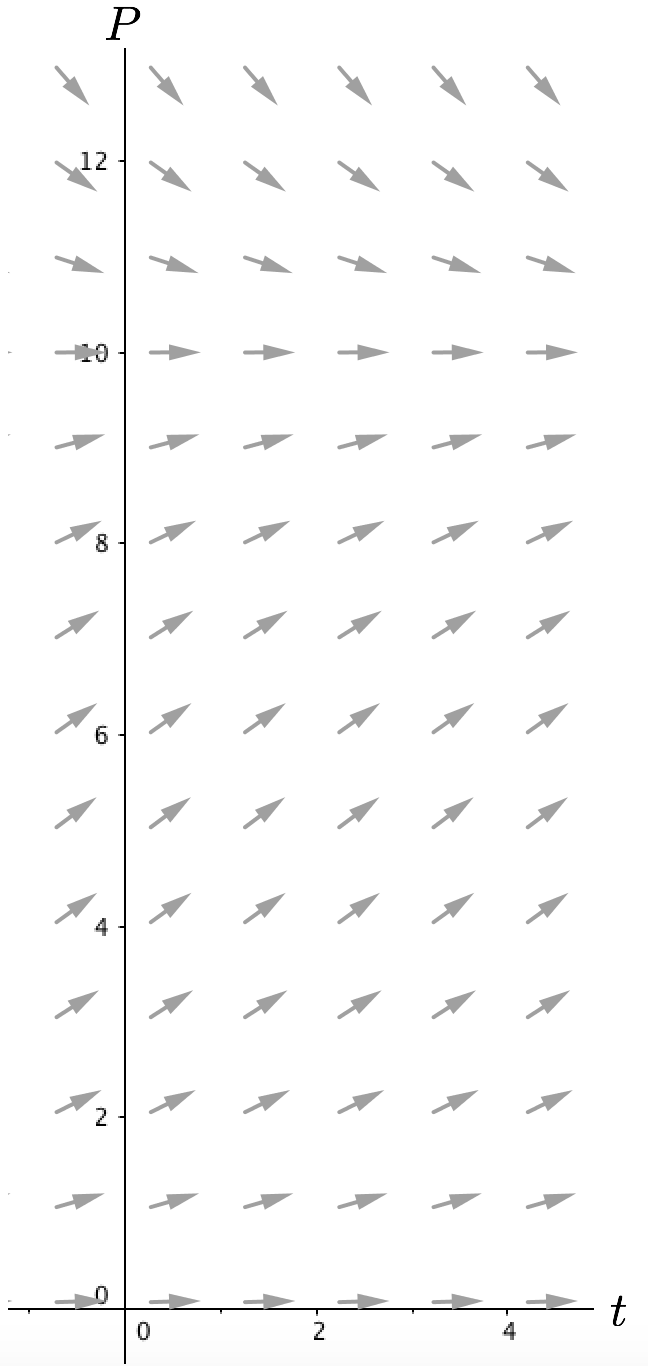
\includegraphics[width=2in]{03/03SlopeFieldFish.png}
\end{center}
 
\begin{enumerate}[resume]
\item \label{03problem2}
\begin{enumerate}
\item On the slope field above, stitch together in a tip to tail manner several tangent vectors to produce a graph of the population versus time if at time $t = 0$ we know there are 8 fish in the lake (again, think of 8 as scaled for say, 8000 or 80,000). \label{03problem3parta}
\vs
\item Reproduce your technique as much as possible using the Slope Field Stitcher applet, \\ \href{https://ggbm.at/FZn4WHeU}{\underline{https://ggbm.at/FZn4WHeU}}.  You can use the arrow buttons to move the initial vector around, and then create subsequent vectors to stitch on using the appropriate button. \label{03problem3partb}

\vspace{-.3in}\hspace{-0.75in}
\includegraphics[width=0.5in]{03/03SlopeFieldStitcherQR.png}
\end{enumerate}

\item	Explain how you are thinking about rate of change \textbf{in your method}. For example, is the rate of change constant over some increment? If yes, over what increment? If no, is the rate of change always changing? \label{03problem4}
\vfill

\clearpage

\item Using the differential equation $\displaystyle\frac{dP}{dt}=P\left(1-\frac{P}{20}\right)$ and initial condition $P(0) = 10$, Jos{\'e} and Julie started the following table to numerically keep track of their tip-to-tail method for connecting tangent vectors. Explain Jos{\'e}'s and Julie's approach and complete their table. \textbf{Round to two decimal places.} \label{03problem5}

{
\renewcommand{\arraystretch}{1.5}
\newcolumntype{R}{>{\centering\arraybackslash}X}%
\begin{tabularx}{.4\textwidth}{ |R|R|R| }
\hline
$t$ & $P$ & $\frac{dP}{dt}$\\\hline
0 & 10 & 5\\\hline
0.5 & 12.5 & \\\hline
1.0&&\\\hline
1.5&&\\\hline
\end{tabularx}}
\vfill

\item	Using the same differential equation and initial condition as Jos{\'e} and Julie, Derrick and Delores started their table as shown below. Explain how Derrick and Delores' approach is different from Jos{\'e} and Julie's and then complete their table. \textbf{Round to two decimal places.} \label{03problem6}

{
$\displaystyle  \frac{dP}{dt}=P\left( 1-\frac{P}{20}\right) $
 
\renewcommand{\arraystretch}{1.5}
\newcolumntype{R}{>{\centering\arraybackslash}X}%
\begin{tabularx}{.4\textwidth}{ |R|R|R| }
\hline
$t$ & $P$ & $\frac{dP}{dt}$\\\hline
0 & 10 & 5\\\hline
.25 & 11.25 & \\\hline
.5&&\\\hline
.75&&\\\hline
\end{tabularx}}
\vfill

\item Which approach do you think is more accurate and why? \label{03problem7}
\vfill

\clearpage

\item
\begin{enumerate}
\item Consider the differential equation $\displaystyle\frac{dy}{dt}=y+t$ and initial condition $y(0) = 4$. Use Jos{\'e} and Julie's approach to find $y(1.5)$. Show your work graphically and in a table of values. \label{03problem8parta}
\vfill
\vfill
\item Is your value for $y(1.5)$ the exact value or an approximate value? Explain. \label{03problem8partb}
\vfill
\end{enumerate}
\item	\textbf{Generalizing your tip-to-tail approach}. Create an equation-based procedure/algorithm that would allow you to predict future $y$-values for any differential equation $\displaystyle\frac{dy}{dt}$, any given initial condition, and any time increment. \label{03problem9} \vfill \vfill

\end{enumerate}

